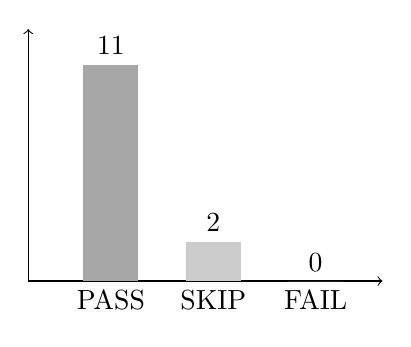
\begin{tikzpicture}[x=1cm, y=1cm]
  \def\barwidth{0.7}
  \def\scale{0.25}

  % Axes
  \draw[->] (0,0) -- (4.5,0);
  \draw[->] (0,0) -- (0,3.2);

  % PASS=11, SKIP=2, FAIL=0
  \fill[gray!70] (0.7,0) rectangle +( \barwidth, {11*\scale} );
  \fill[gray!40] (2.0,0) rectangle +( \barwidth, {2*\scale} );
  \fill[gray!20] (3.3,0) rectangle +( \barwidth, {0*\scale} );

  \node[below] at (1.05,0) {PASS};
  \node[below] at (2.35,0) {SKIP};
  \node[below] at (3.65,0) {FAIL};

  \node[above] at (1.05,{11*\scale}) {11};
  \node[above] at (2.35,{2*\scale}) {2};
  \node[above] at (3.65,0) {0};
\end{tikzpicture}
